\documentclass{beamer}
%\usepackage[all,arc,curve,frame,color]{xy}
%\usepackage{tkz-graph}
\usepackage{mathtools}
\usepackage{ragged2e,etoolbox}


\newenvironment{nstabbing}
  {\setlength{\topsep}{0pt}%
   \setlength{\partopsep}{0pt}%
   \tabbing}
  {\endtabbing}

\def\jump{ \quad \\ \vspace{0.7cm} \pause}
\newcommand{\nc}{\newcommand}
\nc{\pid}{\mathfrak{p} }
\nc{\dpid}{\delta_{\mathfrak{p}}}

\def\AA{{\mathbb A}}
\def\CC{{\mathbb C}}
\def\EE{{\mathcal E}}
\def\FF{{\mathcal F}}
\def\GG{{\mathcal G}}
\def\HH{{\mathcal H}}
\def\MM{{\mathcal M}}
\def\NN{{\mathbb N}}
\def\PP{{\mathbb P}}
\def\QQ{{\mathbb Q}}
\def\RR{{\mathbb R}}
\def\ZZ{{\mathbb Z}}
\def\aa{{\mathbf a}}
\def\bb{{\mathbf b}}
\def\del{\partial}
\def\kk{\Bbbk}
\def\mm{{\mathfrak m}}
\def\nn{{\mathfrak n}}
\def\pp{{\mathfrak p}}
\def\qq{{\mathfrak q}}
\def\rr{{\mathbf r}}
\def\uu{{\mathbf u}}
\def\vv{{\mathbf v}}
\def\ww{{\mathbf w}}
\def\xx{{\mathbf x}}
\def\yy{{\mathbf y}}
\def\zz{{\mathbf z}}
\newcommand{\PGL}{\textrm{PGL}}
\newcommand{\res}{\textrm{Res}}


\DeclareMathOperator{\Tail}{Tail}
\DeclareMathOperator{\Per}{Per}
\DeclareMathOperator{\PrePer}{PrePer}
\DeclareMathOperator{\HTail}{HTail}
\DeclareMathOperator{\HPer}{HPer}
\DeclareMathOperator{\HPrePer}{HPrePer}

\makeatletter
\def\th@mystyle{%
    \normalfont % body font
    \setbeamercolor{block title example}{bg=orange,fg=white}
    \setbeamercolor{block body example}{bg=orange!20,fg=black}
    \def\inserttheoremblockenv{exampleblock}
  }
\makeatother

\makeatletter
\def\th@thmstyle{%
    \normalfont % body font
    \setbeamercolor{block title example}{bg=blue,fg=white}
    \setbeamercolor{block body example}{bg=blue!20,fg=black}
    \def\inserttheoremblockenv{exampleblock}
  }
\makeatother

\definecolor{darkgreen}{RGB}{77,153,0}
\makeatletter
\def\th@qstnstyle{%
    \normalfont % body font
    \setbeamercolor{block title example}{bg=darkgreen,fg=white}
    \setbeamercolor{block body example}{bg=green!20,fg=black}
    \def\inserttheoremblockenv{exampleblock}
  }
\makeatother

\theoremstyle{thmstyle}
\newtheorem*{mydef}{Definition}

\theoremstyle{thmstyle}
\newtheorem*{mythm}{Theorem}

\theoremstyle{mystyle}
\newtheorem*{remark}{Remark}
\newtheorem*{conjecture}{Conjecture}
\newtheorem*{mycor}{Corollary}
\newtheorem*{mylemma}{Lemma}

\theoremstyle{qstnstyle}
\newtheorem*{question}{Question}

\usepackage{remreset}% tiny package containing just the \@removefromreset command
\makeatletter
\@removefromreset{subsection}{section}
\makeatother
\setcounter{subsection}{1}

\newcommand\Wider[2][3em]{%
\makebox[\linewidth][c]{%
  \begin{minipage}{\dimexpr\textwidth+#1\relax}
  \raggedright#2
  \end{minipage}%
  }%
}

\mode<presentation>{\usetheme{CambridgeUS}\usecolortheme{dolphin}} 
%\setbeamertemplate{navigation symbols}{}
\setbeamertemplate{blocks}[rounded][shadow=false]


\title[Bounds for Preperiodic Points]{Bounds for Preperiodic Points for Rational Maps with Good Reduction}
%\subtitle[Dissertation Defense]{Dissertation Defense}
\author[S. Troncoso]{Sebastian Troncoso}
\institute[BSC]{Birmingham-Southern College}
%\titlegraphic{\includegraphics[height=1.5cm]{../images/normale_pisa.png}}
\date[September 25, 2017.]{ September 25, 2017. \\ \vspace{1cm} }


%\AtBeginSection[]{} % for optional outline or other recurrent slide
\AtBeginSection{\frame{\sectionpage}}
\begin{document}

\begin{frame}
\titlepage
\end{frame}

\begin{frame}
\frametitle{Notation}
For simplicity, during this talk we will work with $\mathbb{Q}$ and its ring of integers $\mathbb{Z}$.
\jump
However, the theory is more general than that and $\mathbb{Q}$ and $\mathbb{Z}$ may be replace by a number field and $\mathcal{O}_K$ its ring of algebraic integers.
\jump
Let $\displaystyle \mathbb{P}^1(\QQ)=\{[x:y] \mid  [x:y]\sim [\lambda x:\lambda y] \quad \lambda\in \QQ^{*} \} = \QQ\cup \{\infty \}$ be  the projective line. \pause When we write $\PP^1$ is assume to be $\PP^1(\CC)$.

\end{frame}

\begin{frame}
\frametitle{Notation}
$\phi:\mathbb{P}^1\to\mathbb{P}^1$ be an endomorphism defined over $\QQ$.
\jump
$\phi([x:y])=[F(x,y):G(x,y)]$ where $F$ and $G$ are polynomials of the same degree with coefficients in $\QQ$ and with no common zeros.
\jump
$\displaystyle\phi(x)=\frac{f(x)}{g(x)}$ where $f$ and $g$ are polynomials with coefficients in $\QQ$.
\jump
$\phi^n$ is the $n$th iterate of $\phi$.
\\ \pause
The \textbf{orbit} of a point $P\in\PP^1$ is the set 
$$ O_{\phi}(P) = \{P, \phi(P),\phi^2(P),\phi^3(P),\ldots \}.$$

\pause The \textbf{orbit length} of $P$ is the cardinality of the orbit of $P$ (as a set).
\end{frame}

\begin{frame}
\frametitle{Notation}

\textbf{Periodic point}: $\phi^n(P)=P$ for some $n\geq{1}$.
\\\quad\quad \pause Minimal $n$ is called the \textbf{period} of $P$.

\pause
\vspace{2mm}
The set of rational periodic points for $\phi$ is denoted by $\Per(\phi,\QQ)$.
\\\quad\\
\pause
\textbf{Preperiodic point}: $\exists m\geq{0}$ such that $\phi^m(P)$
is periodic \\\quad\quad \pause \emph{i.e.}  $P$ has finite orbit.

\pause
\vspace{2mm}
The set of rational preperiodic points for $\phi$ is denoted by $\PrePer(\phi,\QQ)$.
\\\quad\\
\pause
\textbf{Tail point}: A point that is preperiodic but not periodic.

\pause
\vspace{2mm}
The set of $\QQ$-rational tail points for $\phi$ is denoted by $\Tail(\phi,\QQ)$.
\end{frame}

\begin{frame}
\frametitle{Examples:}
$\PP^1(\QQ)=\QQ\cup \{\infty \}$ and endomorphism of $\PP^1$ as rational functions. Consider $\phi_c(z)=z^2+c$.
\pause

\begin{center}
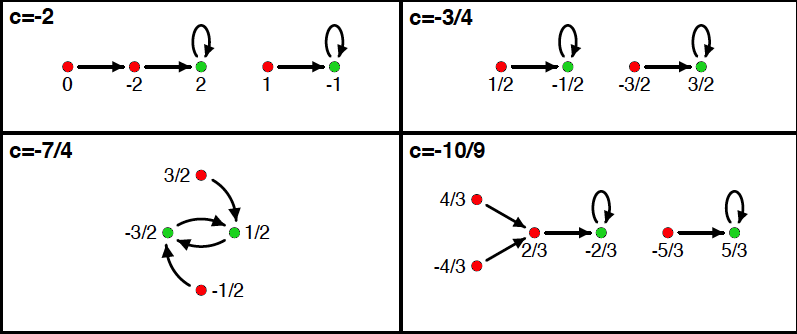
\includegraphics[width=1.0\linewidth]{placeholder4}
\end{center}

rational tail points (red) and rational periodic points (green) of  $\phi_c(z)=z^2+c$.
\end{frame}

\begin{frame}
\frametitle{Question:}
\begin{itemize}
\item Are the sets $\Tail(\phi,\QQ)$, $\Per(\phi,\QQ)$ and $\PrePer(\phi,\QQ)$ finite? 
\end{itemize}
\pause \textbf{Yes}. 
\vspace{6mm}\pause

\begin{mythm}[Northcott 1950]
Let $\phi : \PP^1 \to \PP^1$ be an endomorphism of degree $\geq{2}$
defined over $\QQ$. Then $\phi$ has
only finitely many preperiodic points in $\PP^1(\QQ)$.
\end{mythm}

\vspace{6mm} \pause
We can deduce from the original proof of Northcott's theorem a bound for $|\PrePer(\phi,\QQ)|$ depending on
\begin{itemize}
\item the degree of $\phi$
\item height of the coefficients of $\phi$


 
\end{itemize}
\end{frame}

\begin{frame}
\frametitle{Goals:}
Give explicit bounds for $|\Tail(\phi,\QQ)|$, $|\Per(\phi,\QQ)|$ and $|\PrePer(\phi,\QQ)|$ in terms of:\pause
\begin{itemize}
\item The degree $d$ of $\phi$.
\end{itemize}

\pause

\begin{conjecture}[Uniform Boundedness Conjecture - Morton--Silverman
  1994]
There exists a bound $B = B(d)$ such that if $\phi:\mathbb{P}^1\rightarrow\mathbb{P}^1$ is an endomorphism of degree $d\geq{2}$ defined over $\QQ$, then 
$$|\text{PrePer}(\phi,\QQ)| \leq B.$$
\end{conjecture}
\end{frame}

%\begin{frame}
%The conjecture Uniform Boundedness Conjecture (UBC) is an extremely strong uniformity conjecture.
%\jump
%\begin{itemize}
%\item The UBC on maps of degree $4$ on $\PP^1$ defined over $\QQ$ implies Mazur's theorem that the rational torsion subgroup of
%an elliptic curve $E/\QQ$ is bounded independently of $E$.
%\jump
%\item The UBC for maps of degree $4$ on $\PP^1$ defined over $K$ implies Merel's theorem that the size of the rational torsion subgroup
%of an elliptic curve over a number field $K$ is bounded only in terms of the degree of $[K : \QQ]$.
%\jump
%\item  Lattes maps are the only nontrivial family of rational maps for which the UBC is currently known.
%\end{itemize}
%
%
%\end{frame}


\begin{frame}
\frametitle{Poonen's Conjecture}

The simplest case we could consider for the UBC is \pause  $\phi$ a quadratic polynomial in one variable with coefficients in $\QQ$.

\pause
\vspace{4mm}


\begin{conjecture}[Poonen's Conjecture]
Let $\phi$ be a quadratic polynomial defined over $\mathbb{Q}$ then 
$$|\PrePer(\phi,\QQ)| \leq 9.$$
\end{conjecture}

\pause
\vspace{6mm}

If $\phi=x^2+d$ then B. Hutz and P. Ingram have shown that Poonen's conjecture holds when the numerator and denominator of $d$ don't exceed $10^8$.

\end{frame}

\begin{frame}
\frametitle{Goals:}

In order to get explicit bounds for the cardinality of the set $\PrePer(\phi,\QQ)$ we need an extra parameter. 

Instead of the height of $\phi$ we can use a weaker and more natural parameter to get bound on $|\PrePer(\phi,\QQ)|$.\pause 
\jump
This parameter is the number of primes of bad reduction of $\phi$.
\jump
Give explicit bounds for $|\Tail(\phi,\QQ)|$, $|\Per(\phi,\QQ)|$ and $|\PrePer(\phi,\QQ)|$ in terms of:
\begin{itemize}
\item The degree $d$ of $\phi$.

\item The number of primes of bad reduction of $\phi$.
\end{itemize}
\end{frame}

\begin{frame}
\frametitle{Good/Bad Reduction}

\begin{itemize}
\item Let $\pid$ be a prime in $\ZZ$ and $\phi(x)=\frac{F(x)}{G(x)}$ be a rational function $\PP^1$ defined over $\QQ$. \pause  After multiplying for the common denominator of the coefficients of $F$ and $G$. We may assume that $F$ and $G$ are polynomials with coefficients in $\ZZ$.

\pause
Consider the reduction of $\phi$ modulo $\pid$ given by
$$\tilde{\phi}(x)=\frac{\tilde{F}(x)}{\tilde{G}(x)} $$
In other words, $\tilde{\phi}$ is obtained by reducing the coefficients of $F,G$ modulo $\pid$.
\jump
Then $\phi$ has \textbf{good reduction} at $\pid$ if the degree of $\phi$ is equal to the degree of $\tilde{\phi}$.
\end{itemize}
\end{frame}

\begin{frame}
\frametitle{Good/Bad Reduction}
\begin{itemize}
\item $\phi$ has \textbf{bad reduction} at $\pid$ if it does not have good reduction at $\pid$.
\jump
\item We say that $\phi$  has \textbf{good reduction outside} $S$ if $\phi$ has good reduction for every $\pid \notin S$.

\jump
\end{itemize}

If we allow the number of primes of bad reduction as a parameter, much more is known for the cardinality of the set of rational preperiodic points. 
\end{frame}



\begin{frame}
\frametitle{Bound on maximal period}
\begin{mythm}[W.\ Narkiewicz 1988]
Let $\phi \in \QQ[z]$ be a polynomial of degree $\geq{2}$ defined over $\QQ$. 
Suppose $\phi$ has good reduction outside a finite set of primes $S$.
\\\quad\\
If $P$ is a rational periodic point of period $n$, then
$$ n \leq (6\cdot 7^{D+2|S|})^\alpha,$$ where $\alpha=O(|S|\log{|S|}).$
\end{mythm}
\end{frame}
%Let $S$  be a finite set of primes of $\ZZ$.



\begin{frame}
\frametitle{Bound on maximal orbit length of a preperiodic point}
\begin{mythm}[J.K.\ Canci 2006]
Let $\phi : \PP^1\to\PP^1$ be a rational map of degree at least two
defined $\QQ$. 
Suppose $\phi$ has good reduction outside a finite set of primes $S$.
\\\quad\\
If $P\in\text{PrePer}(\phi,\QQ)$ is of orbit length $n$, then
$$n\leq\left[{e^{10}}^{12}(|S|+1)^8(log(5(|S|+1)))^8\right]^{|S|}.$$
\end{mythm}
\end{frame}

\begin{frame}
\frametitle{Bound on maximal orbit length of a preperiodic point }
\begin{mythm}[J.K.\ Canci, L.\ Paladino 2015]
Let $\phi : \PP^1\to\PP^1$ be a rational map of degree $\geq{2}$
defined over $\QQ$. Suppose $\phi$ has good reduction outside a finite set of primes $S$ of $\ZZ$.
If $P\in\text{PrePer}(\phi,\QQ)$ is of orbit length $n$, then
$$n\leq \max\left\{(2^{16|S|-8}+3)\left[12|S|\log(5|S|)\right]^{D}, \left[12(|S|+2)\log(5|S|+5)\right]^{4D}\right\}
.$$
\end{mythm}
\jump
From here we can deduce a bound for $|\PrePer(\phi,\QQ)| $ that is roughly of the order $\displaystyle d^{2^{16|S|}\left( |S|\log(|S|) \right)^{D}}$.

\end{frame}

\begin{frame}
\begin{mythm}[S.\ Troncoso 2016]
Let $\phi : \PP^1\to\PP^1$ be a rational map of degree $\geq{2}$
defined over $\QQ$. Suppose $\phi$ has good reduction outside a finite set of primes $S$ of $\ZZ$. Then
\begin{enumerate}
\item [(a)] $|\Per(\phi,\QQ)| \leq  2^{16|S|d^3}+3.$

\item [(b)] $|\Tail(\phi,\QQ)| \leq  4(2^{16|S|d^3}) .$

\item [(c)] $|\PrePer(\phi,\QQ)| \leq 5(2^{16|S|d^3})+3.$

\end{enumerate}
\end{mythm}

Notice that the bounds obtained  in the theorem are a significant improvement from the previous bound given by Canci and Paladino which was of the order $\displaystyle d^{2^{16s}\left( s\log(s) \right)^{D}}$ for the set $|\PrePer(\phi,\QQ)|$.
\end{frame}


\begin{frame}
\frametitle{Bounds for Preperiodic points}

The previous theorem use some important results like:\pause
\jump
\begin{itemize}
\item Riemann-Hurwitz formula
\pause
\item  Baker's Theorem on existence of periodic points
\pause
\item Kisaka's analysis on Baker's Theorem
\pause
\item Logarithmic $p$-adic chordal distance.
\pause
\item Study the distance between periodic and tail points.
\pause
\item Number of solution of the $S$-unit equation.
\end{itemize}
\end{frame}


\begin{frame}
\frametitle{Bounds independent of the degree}
\begin{mythm}[S.\ Troncoso 2016]
Let $\phi : \PP^1\to\PP^1$ be a rational map of degree $\geq{2}$
defined over $\QQ$. Suppose $\phi$ has good reduction outside a finite set of primes $S$ of $\ZZ$.
\begin{enumerate}

\item [(a)] 
If there are at least three rational tail points of $\phi$ then
$$|\Per(\phi,\QQ)| \leq 2^{16|S|}+3. $$

\item [(b)]
If there are at least four rational periodic points of $\phi$ then
$$|\Tail(\phi,\QQ)| \leq 4(2^{16|S|}).$$
\end{enumerate}
\end{mythm}
\end{frame}


\begin{frame}
\frametitle{$S$-unit equations}
Let $S$ be a finite set of primes of $\ZZ$ and $\ZZ_S^{*}$ be the group of $S$-units \emph{i.e.} $\ZZ_S^{*}$ is the set of fraction of the form $\displaystyle\frac{a}{b}$ where $a$ and $b$ are not divisable by primes in $S$.\pause

\begin{itemize}

\item A linear relation of the form $$au+bv=1$$  where  $(u,v) \in \left(\ZZ_S^*\right)^2$ and $a,b\in \QQ^{*}$ is called a $S$-unit equation. \pause
\item Beukers and Schlickewei give an explicit bound  for the $S$-unit equation. The number of solutions $(u,v) \in \left(\ZZ_S^{*}\right)^2$ to 
$$au+bv=1$$ 
is bounded by $$2^{8(2|S|+2)}.$$
\end{itemize}
\end{frame}



\begin{frame}
\frametitle{Almost ready project}
Joint work with J.K.\ Canci and S.\ Vishkautsan \\
\pause
\begin{mythm}[S.\ Troncoso 2016]
Let $S$  be a finite set of primes of $\ZZ$. Let $\phi$ be an endomorphism of $\PP^1$, defined over $\QQ$, and $d\geq 2$ the degree of $\phi$. Assume $\phi$ has good reduction outside $S$. Then 
$$|{\rm PrePer}(\phi,\QQ)| \leq \kappa_1 d^2+\lambda_1$$

If we assume that $\phi$ has a rational periodic point of minimal period at least two then
$$|{\rm PrePer}(\phi,\QQ)| \leq \kappa_2 d+\lambda_2.$$
\end{mythm}
\pause 

We emphasize that the constants $\kappa_1,\kappa_2,\lambda_1$ and $\lambda_2$ in the theorem depend only on the cardinality of $S$. An explicit definition of the constants $\kappa_1,\kappa_2,\lambda_1$ and $\lambda_2$ can be given.
\end{frame}


\begin{frame}
\frametitle{Current project}

\Huge{Arithmetic dynamics in $\PP^n$}
\end{frame}

\begin{frame}
\Huge{THANK YOU}
\end{frame}


\end{document}
